\section{SReach algorithm}
The main idea implemented in {\it SReach} is to use a set of random variables to encode all the stochastic information first. In detail, when a hybrid automaton is given, {\it SReach} directly declares each probabilistic system parameter as one random variable with a known distribution. While for a PHA, each probabilistic guarded command $g \rightarrow p_1:u_1 + \cdots + p_m:u_m$ is rewritten by introducing a new random variable $rv$ such that $Pr(rv = i) = p_i$. For example, a probabilistic command $x \geq 1 \to 0.7 : (x' = 1)+ 0.3 :( x' = x)$ will be rewritten as two new guarded commands after introducing a new random variable $r$ whose distribution is $(Pr(r=1)=0.7, Pr(r=2)=0.3)$. One is $x \geq 1 \wedge r = 1 \to x'=1$. The other is $x \geq 1 \wedge r = 2 \to x'=x$. When additional randomness is involved in assigning probabilities for probabilistic transitions or in resetting system variables, addtional random variables are needed. For instance, {\it SReach} can express a probabilistic guarded command as $x \geq 1 \to p_1 : (x' = p_2 )+ (1-p_1) :( x' = x)$, where $p_1$ is a random variable which obeys to an Uniform distribution from 0.6 to 0.85, and $p_2$ is a random variable whose distribution is $N(0,1)$.

After encoding all the stochastic elements using random variables, {\it SReach} samples all random variables according to their probability distributions. For each sampled assignment to these random variables, we obtain a corresponding hybrid automaton by replacing all random variables with assigned values. Then, the bounded model checker for hybrid automata {\it dReach} \cite{gaodelta} is adapted to analyze each obtained hybrid automaton $M_i$, together with the desired precision $\delta$ and the unfolding steps $k$. {\it dReach} returns either unsat or $\delta$-sat for $M_i$ (see Appendix \ref{apndx:dreach} for more on the $\delta$-complete decision procedures). This information
is then used by statistical tests to decide whether to stop or to repeat the procedure. The full procedure is illustrated in Algorithm \ref{fig:sreach}, where $MP$ is a given probabilistic model, and $ST$ indicates which statistical testing method will be used. $Succ$ is used to record the number of $\delta$-sat instances that are returned by {\it dReach}, and $N$ the total of samples generated so far. These two numbers are then the inputs of {\it SReach}'s statistical testing procedure $ST$. Since the full nondeterminism within obtained hybrid automata has been considered when handling the bounded reachability problems, the estimated probabilities computed by {\it SReach} are the maximum probabilities. Also, for a probabilistic hybrid automaton, sampling and fixing all the probabilistic transitions in advance results in an over-approximation of the original probabilistic model. Because the result is an over-approximation, safety properties are preserved. To improve the performance of {\it SReach}, each sampled assignment, together with its corresponding {\it dReach} result, has been recorded for avoiding repeated calls of {\it dReach} with the same sampled assignments. This significantly reduces the total calls to {\it dReach} for PHAs without additional randomness, as the size of sample space is comparatively small. For the example PHA, as shown in Figure \ref{fig:examplepha}, with this improvement, the total checking time for a reachability problem with $k=2$ has been decreased from $11291.31$s for $658$ samples ($17.16$s per sample) to $3295.82$s ($5.01$s per sample). To further improve the performance, a parallel version of {\it SReach} has been implemented, where multiple samples and corresponding hybrid automata are generated, and passed to {\it dReach} simultaneously. Using this parallel version of {\it SReach} on a four-core machine, the running time for the above example PHA has been further decreased to $2119.55s$ for $660$ samples ($3.33$s per sample). 
\begin{figure}
\centering
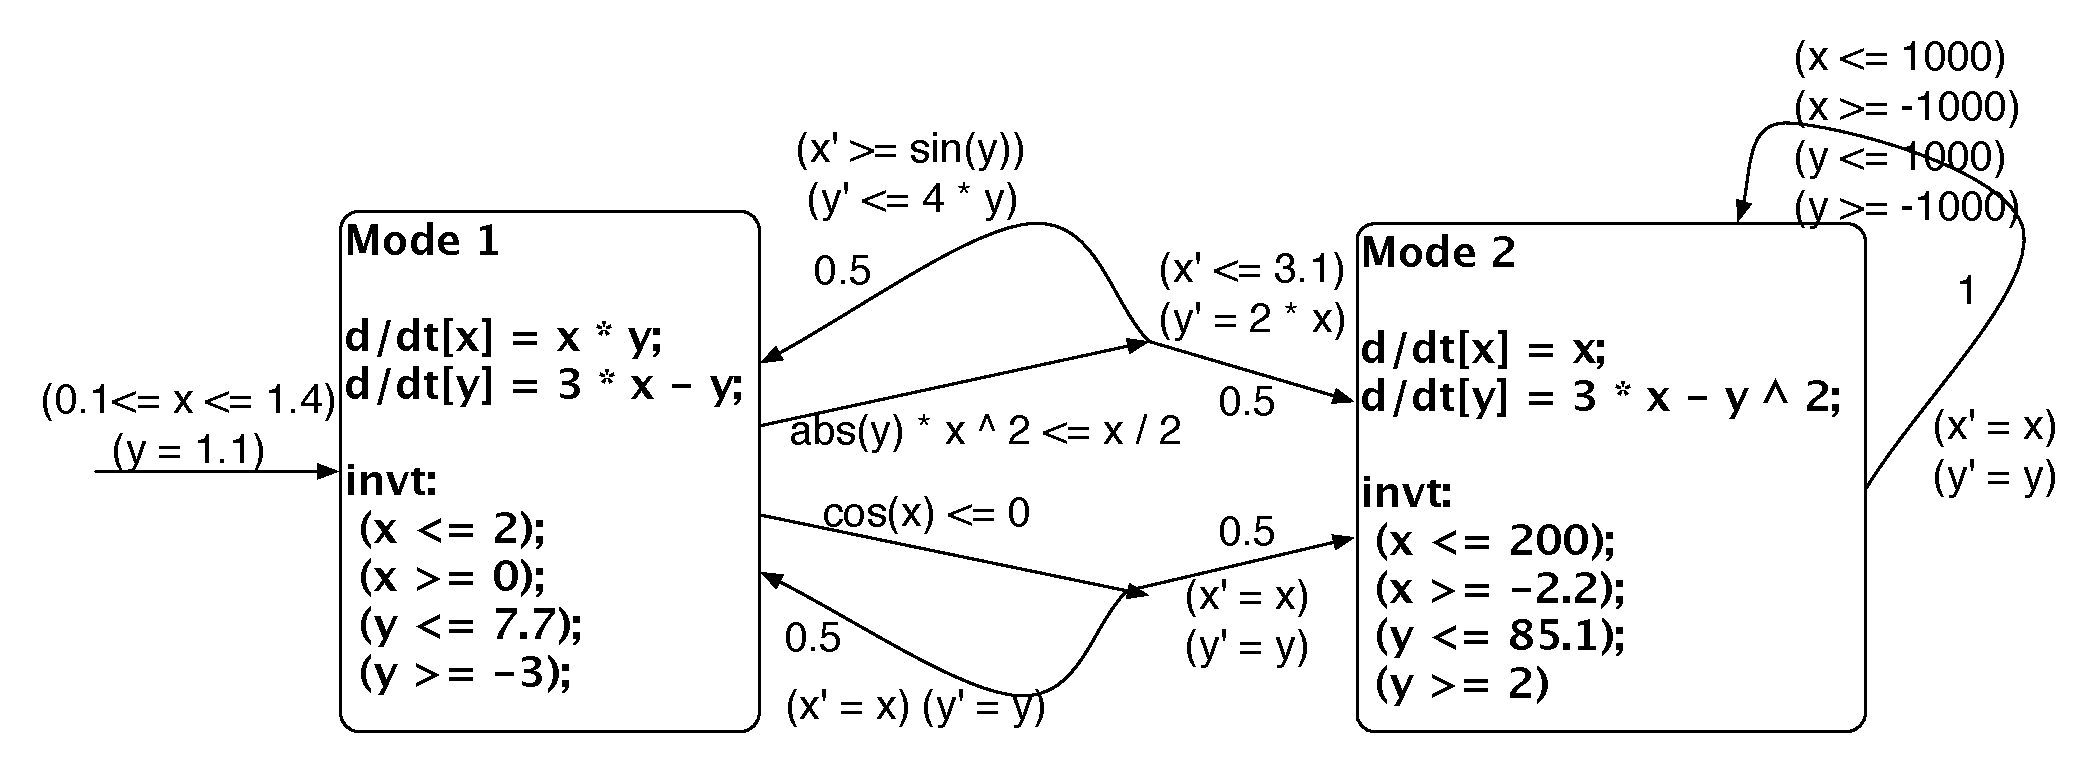
\includegraphics[width=\linewidth]{examplepha}
\caption{An example probabilistic hybrid automaton}
\label{fig:examplepha}
\end{figure}


\begin{algorithm}
  \centering
  \caption{SReach}
  \label{fig:sreach}
  \begin{algorithmic}[1]
    \Function{SReach}{$MP$, $ST$, $\delta$, $k$}
        \State $Succ \gets 0$	\Comment{number of $\delta$-sat samples}
        \State $N \gets 0$	\Comment{total number of samples}
        \State $RV \gets \mathrm{ExtractRV}(MP)$	\Comment{get the RVs from the probabilistic model}
        \Repeat
            \State $S_i \gets \mathrm{Sim}(RV)$		\Comment{sample the parameters}
            \State $M_i \gets \mathrm{Gen}(MP, S_i)$	\Comment{generate a dReach model}
            \State $Res \gets \mathrm{dReach}(M_i, \delta, k)$	\Comment{call dReach}
            \If{$Res$ = $\delta$-sat}
            	%Good
		\State $Succ \gets Succ + 1$
%	  \Else
%	   	%Bad
%		\State $Fail \gets Fail + 1$
	    
	  \EndIf
	\State $N \gets N + 1$
        \Until{$ST.done(Succ, N)$}	\Comment{perform statistical test}\\
        %\State $Est\_prob \gets Succ / N$
	\quad\hspace{0.5ex} \Return $ST.output$
   \EndFunction
  \end{algorithmic}
\end{algorithm}

Currently, {\it SReach} supports a number of hypothesis testing and statistical estimation techniques including: the {Lai's test} \cite{lai1988nearly}, {Bayes factor test} \cite{kass1995bayes}, {Bayes factor test with indifference region} \cite{younes2005verification}, {Sequential probability ratio test (SPRT)}\cite{wald1945sequential}, {Chernoff-Hoeffding bound} \cite{hoeffding1963probability}, {Bayesian Interval Estimation with Beta prior}\cite{zuliani2010bayesian}, and {Direct Sampling}. All methods produce answers to some correctness precision that can be set arbitrarily by the user. See Appendix \ref{apndx:stat} for more details about how these tests can guarantee an arbitrary small error bound between the estimated probability and the real one. With these hypothesis testing methods, {\it SReach} can answer qualitative questions, such as ``Does the model satisfy a given reachability property in $k$ steps with probability greater than a certain threshold?'' While with the above statistical estimation techniques, {\it SReach} can offer answers to quantitative problems. For instance, ``What is the probability that the model satisfies a given reachability property in $k$ steps?''  {\it Sreach} can also handle additional types of interesting problems by encoding them as bounded reachability problems. The {\bf model validation} problem with prior knowledge can be encoded as a bounded reachability question. Expressing prior knowledge about the given model as reachability properties, is there any number of steps $k$ in which the model satisfies a given property? If none exists, the model is incorrect regarding the given prior knowledge. If, for each property, a witness is returned, we can conclude that the model is correct with regard to the prior knowledge. The {\bf parameter estimation} problem can also be encoded as a $k$-step reachability problem. Does there exist a parameter combination for which the model reaches the given goal region in $k$ steps? If so, this parameter combination is potentially a good estimation for system parameters. The goal here is to find an assignment with which all the given goal regions can be reached in a bounded number of steps. Moreover, the {\bf sensitivity analysis} can be conducted by a set of bounded reachability queries as well. Are the results of reachability analysis the same for different possible values of a certain system parameter? If so, the model is insensitive to this parameter with regard to the given prior knowledge.


